%****************************************************
%	CHAPTER 2 - LIT REVIEW
%****************************************************
\chapter{Literature Review}
\label{ch:lit_review}

%\begin{itemize}
%    \item Antarctica and the Southern Ocean
%    \item Pancake Ice
%    \item Ocean Waves
%    \item Sea Ice-Environment Interactions
%    \item LIDAR
%\end{itemize}


%====================================================
\section{Antarctica and the Southern Ocean}
\label{sec:ch2.section1}
%----------------------------------------------------

Historically, Antarctica and the Southern Ocean that surrounds it have been neglected by the global scientific community \cite{kennicuttSustainedAntarcticResearch2019}. There are many reasons for this neglect, ranging from the extreme isolation and difficulty associated with reaching the continent, incredibly harsh environmental conditions, and the bias towards the Northern Hemisphere often seen in scientific research. In recent years this has begun to change, with efforts such as the Southern oCean seAsonaL Experiment (SCALE) conducting more regular observations and data collection in the region.

The Earth's environment is a massively complex and interconnected system something something. Without a full understanding of each part of the system, it is impossible to fully understand, model or predict it. The Antarctic Continent, the ice shelf surrounding it, the Marginal Ice Zone (MIZ) and the Southern Ocean are huge parts of this system that are barely understood.


%----------------------------------------------------
\subsection{Antarctic Sea Ice}

Unlike the Arctic, the most common type of sea ice in the Antarctic is not sheet ice  \cite{SeaIce}. The Antarctic climate is far more dynamic with rough seas and cyclones common throughout the year *I'm guessing, must find reference*. These turbulent environmental conditions result in a wider range of sea ice being commonplace in the region. The type of ice present in or on the ocean impacts the climate of the area. Wind and wave activity travels though and is attenuated differently by the many kinds of ice in the region.

%----------------------------------------------------
\subsection{Marginal Ice Zone (MIZ)}
The Marginal Ice Zone (MIZ) is widely accepted to be the area where the open ocean transitions to consolidated ice cover. There is no universally accepted definition of the MIZ, which leads to difficulties in understanding and comparing studies on the area by different authors who have different definitions of the MIZ. Vichi \cite{vichiIndicatorSeaIce2022} states the MIZ is generally seen as the region where sea ice concentration is between 15\% and 80\%, but argues that a simple threshold based definition is limiting. They propose an alternative indicator, based on the statistical variability of sea ice concentration in the region.

Various different types of ice make up the MIZ, but specifics of the types and their concentrations are not fully characterised \cite{vichiIndicatorSeaIce2022}. *somehow link to wave activity and attenuation*
It is known that ocean surface waves are attenuated by sea ice as the waves travel through the MIZ \cite{williamsWaveIceInteractions2013}


%====================================================
\section{Antarctic Seasonal Ice Cycle}
\label{sec:ch2.section2}
%----------------------------------------------------

Add cycle stuff here

%----------------------------------------------------
\subsection{Pancake Ice}

Pancake Ice is the name given to roughly circular, consolidated ice floes commonly found in polar marginal ice zones where wave and wind activity is present.

%----------------------------------------------------
\subsection{Pancake Ice Formation}

Wave activity and, to a lesser degree, wind activity are necessary for the formation of pancake ice, as the continuous motion provided by the wind and waves promotes the formation of frazil and grease ice over nilas ice \cite{shenConceptualModelPancakeice2001}. This prevents continuous sheets of ice from forming over the ocean.

Shen, Ackley and Hopkins \cite{shenConceptualModelPancakeice2001} propose a three-stage model of pancake ice formation:
\begin{enumerate}
    \item Grease-ice stage
    \item Pancake formation stage
    \item Composite pancake stage
\end{enumerate}

%----------------------------------------------------
\begin{figure}[H]
    \centering
    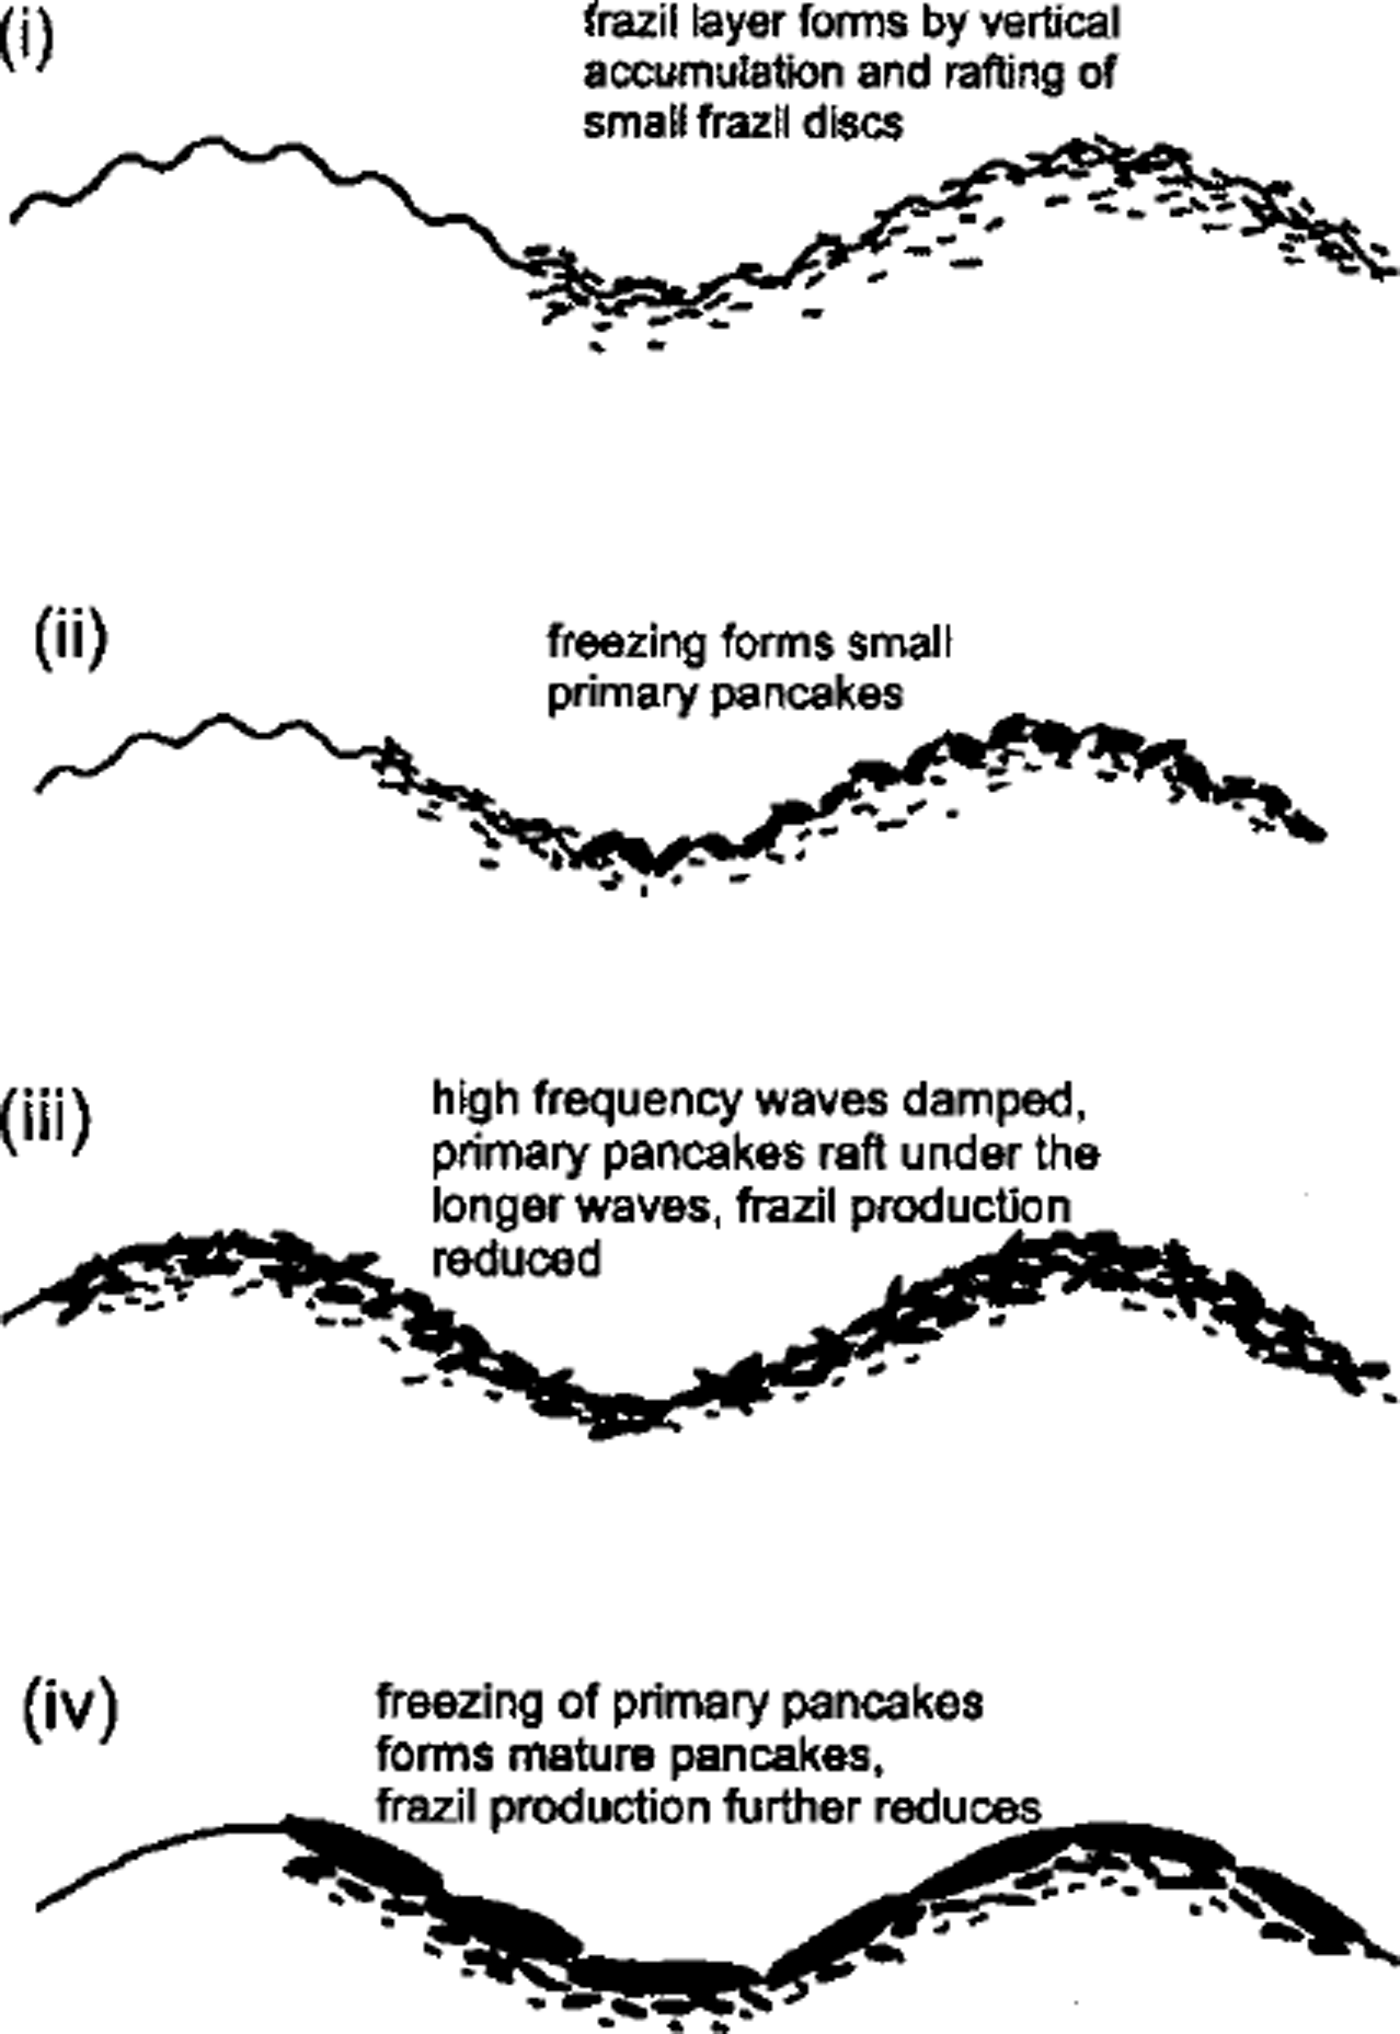
\includegraphics[width=0.4\textwidth]{figs/pancake_formation.png}
    \caption{\textbf{Pancake ice formation process.}}
    \label{fig:pancake_formation}
\end{figure}
%----------------------------------------------------

In the grease-ice stage, the ocean is supercooled, leading to the formation of frazil crystals. Wind and/or wave agitation causes these frazil crystals to collide and adhere to each other, forming miniature disc-like frazils. These newly formed frazils are driven together by the high-frequency components of the wave spectrum to form grease ice, which absorbs the energy of the high-frequency components.

Frazils continue to form and adhere to each other beneath the grease ice layer in the pancake formation stage, leading to an increase in the buoyancy of the accumulated crystals. This increased buoyancy causes the disk-like frazils to rise, exposing them to cold air above the surface of the ocean, resulting in the formation of an ice sheet. Throughout this, the wave motion limits the pancake footprint size and floe-floe collisions result in the formation of ridged edges. The high frequency components of the wave spectrum initially dictate the size of the pancake floes, as the energy from these frequencies is consumed by interactions such as collisions and rafting, lower frequencies begin to drive floe creation and interaction. These lower frequencies result in larger pancake floes being able to form.

In the composite pancake stage, pancakes are driven together by the higher frequency wave components in the same way as the disk-like frazils were in the grease-ice stage. This leads to rafting of the pancakes and freezing between individual rafted pancakes forms composite pancake floes. The production of pancake floes and composite floes will continue until all the wave energy is consumed, leading to a sheet of composite floes. If the wave energy is too great to be absorbed by the floes, the floe size will be limited, and no ice sheet will form.

%====================================================
\section{Ocean Waves}
\label{sec:ch2.section3}
%----------------------------------------------------
The Ocean waves found in the MIZ are wind waves and gravity waves, with wind waves driving most activity.

%----------------------------------------------------
\subsection{Wave Formation}



%====================================================
\section{Sea Ice-Environment Interactions}
\label{sec:ch2.section4}
Sea ice interacts with its immediate environment in various different ways, with the physical structure of the ice having the largest impact on the type and extent of interactions.
Ice both reflects and transmits light, impacts environmental temperature, can damp waves, interact with wind, and by freezing and melting can change the chemical composition of the surrounding seawater.

%----------------------------------------------------
\begin{figure}[H]
    \centering
    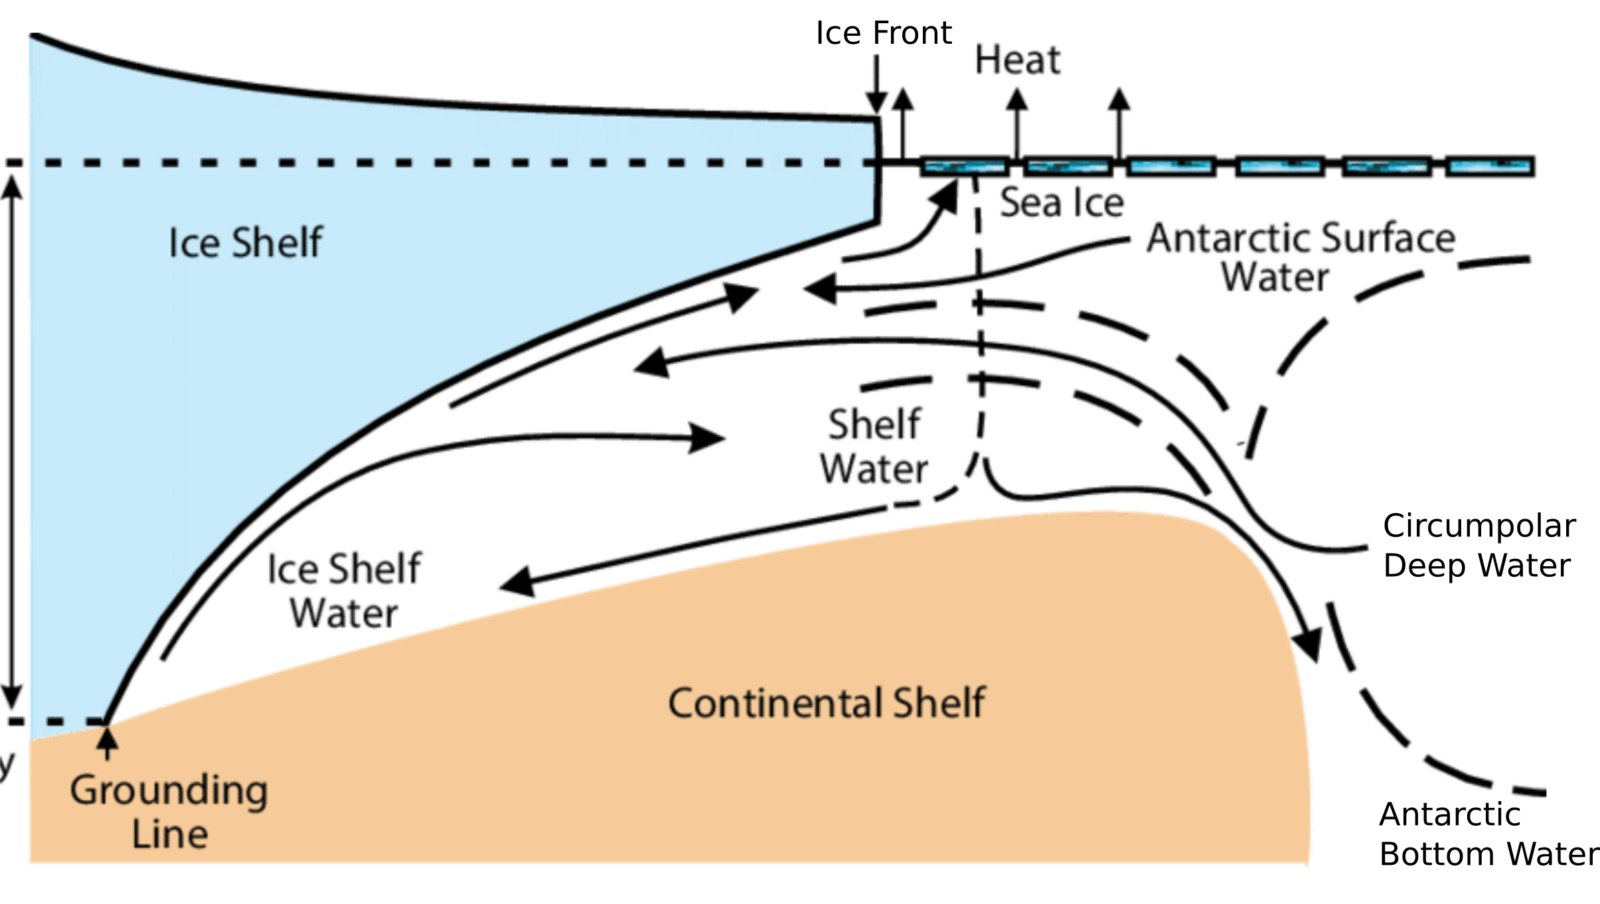
\includegraphics[width=0.7\textwidth]{figs/melting-mechanism.png}
    \caption{\textbf{Melting Mechanism.}}
    \label{fig:melting_mechanism}
\end{figure}
%----------------------------------------------------


%====================================================
\section{Antarctica and Remote Sensing}
\label{sec:ch2.section5}
%----------------------------------------------------

Remote sensing has been the most common method for gathering data on the Antarctic region ever since satellite observation became widespread and the standard method for Earth observation and data collection. The methods for data collection has typically taken the form of Synthetic Aparture Radar (SAR) imaging and Optical imaging (\cite{maslanikRemoteSensingAntarctica1990}). The use of lasers and LIDAR in remote sensing is a recent development that has seem limited implementation in the past two decades (\cite{pettorelliSatelliteRemoteSensing2014}).

The first instance of optical imaging of the Antarctic took place in September 1964, when the Nimbus I satellite catured hundreds of greyscale images of the continent and surrounding ocean (\cite{meierNewEstimatesArctic2013}).
The first use of SAR to collect data over the Antarctic used the RADARSAT-1 sattelite through the RADARSAT-1 Antarctic Mapping Project (RAMP), with the first phase of the project being completed in October 1997 (\cite{jezekRADARSAT1AntarcticMapping2002}).
Laser altimetry was first implemented aboard the Ice, Cloud and land Elevation Satellite (ICESat), through the Geoscience Laser Altimeter System (GLAS). ICESat was a dedicated polar observation satellite, with the primary objective of monitoring the polar iche-sheets. The GLAS produced elevation and atmospheric progiles and was launched in 2003, with data collection commencing on February of that year (\cite{schutzOverviewICESatMission2005}).
After the success of ICESat, ICESat-2 was launched in September of 2018, with the Advanced Topographic Laser Altimeter System (ATLAS) aboard the satellite. The ATLAS sensor marked the first time a LIDAR sensor was equiped to an observation satellite (\cite{palmICESat2AtmosphericChannel2021}).

Remote sensing has many advantages, it allows for long term, consistant data collection, large areas can be surveyed without the need for a physical presence in the region of interest and it can be more cost effective than in-situ data collection. A brief comparison of the three main satellite-based remote sensing methods is given in Table \ref{table:sense_comparison} (\cite{agrawalCOMPARATIVEASSESSMENTREMOTE2019}).

\begin{table}[H]
\centering
\resizebox{\linewidth}{!}{%
\begin{tabular}{llll} 
\hline
\multicolumn{1}{c}{\textbf{Variable}} & \multicolumn{1}{c}{\textbf{Optical}} & \multicolumn{1}{c}{\textbf{SAR}} & \multicolumn{1}{c}{\textbf{LIDAR}}  \\ 
\hline
Sensor Type                           & Passive                              & Active                           & Active                              \\ 
\hline
Electromagnetic Range                 & 0.4 $\mu$ m - 1 mm                   & 1 mm - 1 m                       & 250 nm to 10 $\mu$ m                \\ 
\hline
Weather Limitations                   & Cannot penetrate cloud cover         & Can penetrate cloud cover        & Cannot penetrate heavy cloud cover  \\ 
\hline
Area Coverage                         & Large                                & Large                            & Small                               \\ 
\hline
Data Collected                        & Spectral Radiance                    & Backscatter Amplitude  Phase     & Return Range  Intensity             \\ 
\hline
Data Availibility                     & Many datasets                        & Many datasets                    & Few datasets                        \\ 
\hline
Technique Maturity                    & High                                 & Medium                           & Low                                 \\
\hline
\end{tabular}
}
\caption{\textbf{Remote Sensing Techniques Comparison.} }
\label{table:sense_comparison}
\end{table}

Due to their extreme locations, frequent adverse weather and polar night, SAR has become the most common method for observing both the polar regions (\cite{comisoSatelliteRemoteSensing1991}). Despite the limited resources and harsh conditions, SAR has greatly widened our knowledge of the Antarctic, allowing for tracking of sea ice coverage and extent, snow cover storms, biological activity, ice drift and iceberg calving (\cite{maslanikRemoteSensingAntarctica1990}, \cite{dirscherlRemoteSensingIce2020}, \cite{baumhoerRemoteSensingAntarctic2018}).

Currently, remote sensing falls short when attempting to identify the types of ice covering the ocean. SAR imaging can estimate sea ice extent as well as sea ice concentration. Information on the specific types of ice (grease, frazil, nilas, pancake, etc.) is virtually impossible to extract from SAR data alone (\cite{zakhvatkinaSatelliteSARDatabased2019}).

%----------------------------------------------------
\subsection{Light Detection and Ranging (LIDAR)}

Light Detection and Ranging (LIDAR) is an active remote sensing technique that uses laser pulses to create a three-dimensional representation (a point cloud) of the target subject. A point cloud is a collection of discrete data points in a coordinate space. A point cloud is created by a LIDAR sensor by emitting a pulse of laser light in a specified direction towards the target. The pulse is reflected off a surface on the target and returns to the sensor. Using time of flight and the direction in which the pulse was emitted, the distance to the target and its location is calculated. This process is repeated, directing the laser pulse in different directions at the target to form a complete point cloud. *refine here also could use phase shift instead of ToF*

The development of modern LIDAR began with the invention of lasers, which replaced previous measurement systems based on traditional lights and lamps. Once laser technology matured and reached sufficient beam criteria (shape, wavelength), power density and packaging, could the modern LIDAR sensor be possible. 

%----------------------------------------------------
\subsection{LIDAR Sensors}

A basic LIDAR sensor consists of three main components, a laser source, a steering mechanism to direct the laser beam, and a method of detecting the returning laser beam.

(the exact wavelength of the laser depends on the application and manufacturer's intended use), Different lasers are selected for different reasons, such as penetration power, eye safety, measurement accuracy and something. The steering mechanism used determines the field of view, angular resolution and impacts the measurement accuracy of the sensor. Prisms, mirrors and something can be used to steer the laser's direction. 
Most LIDAR sensors are only capable of creating point clouds with a limited number of predetermined scanning patterns. The most common scanning pattern is a rectangular pattern (an N x M grid of points). Sensors designed for automotive or autonomous vehicle use often have 360 degree coverage in their azimuth and a set vertical resolution, commonly using spinning mirrors or prisms to achieve this.

Some LIDAR sensors are capable of measuring multiple returns from a single output pulse \cite{WhatLidarDataArcGIS}. This is possible when the object hit by the laser pulse does not reflect or absorb all the output energy but allows some to pass through itself. If this occurs multiple times for a single laser pulse, and the sensor is capable of detecting all of these returns, it is possible for a sensor to record more returned points than output laser pulses.

%----------------------------------------------------
\begin{figure}[H]
    \centering
    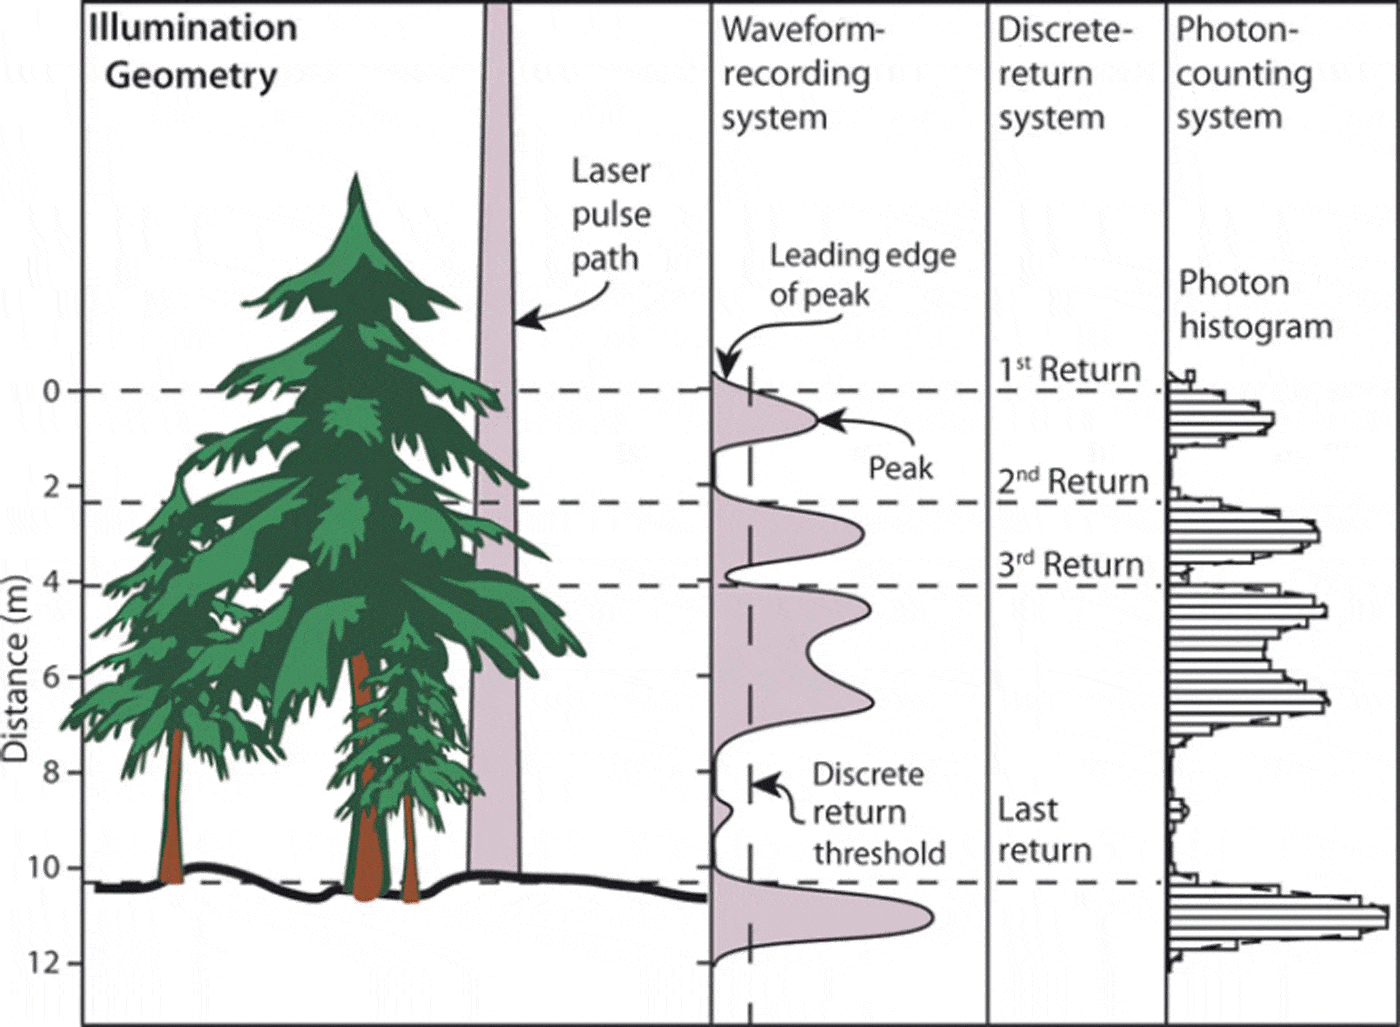
\includegraphics[width=9cm]{figs/multi_return.png}
    \caption{\textbf{Radiation}}
    \label{fig:multi_return}
\end{figure}
%----------------------------------------------------

add mini conclusion

%****************************************************
% END
%****************************************************
